\documentclass{article}

\usepackage{graphicx}
\usepackage{tikz}
\usepackage{tikzsymbols}
\usetikzlibrary{calc,patterns,shapes.geometric}
\pagestyle{empty}
\usepackage[margin=0pt]{geometry}
\geometry{papersize={14in,12in}}

\def\centerarc[#1](#2)(#3:#4:#5){\draw[#1] ($(#2)+({#5*cos(#3)},{#5*sin(#3)})$) arc (#3:#4:#5);}

\begin{document}
	\begin{figure}
		\centering
		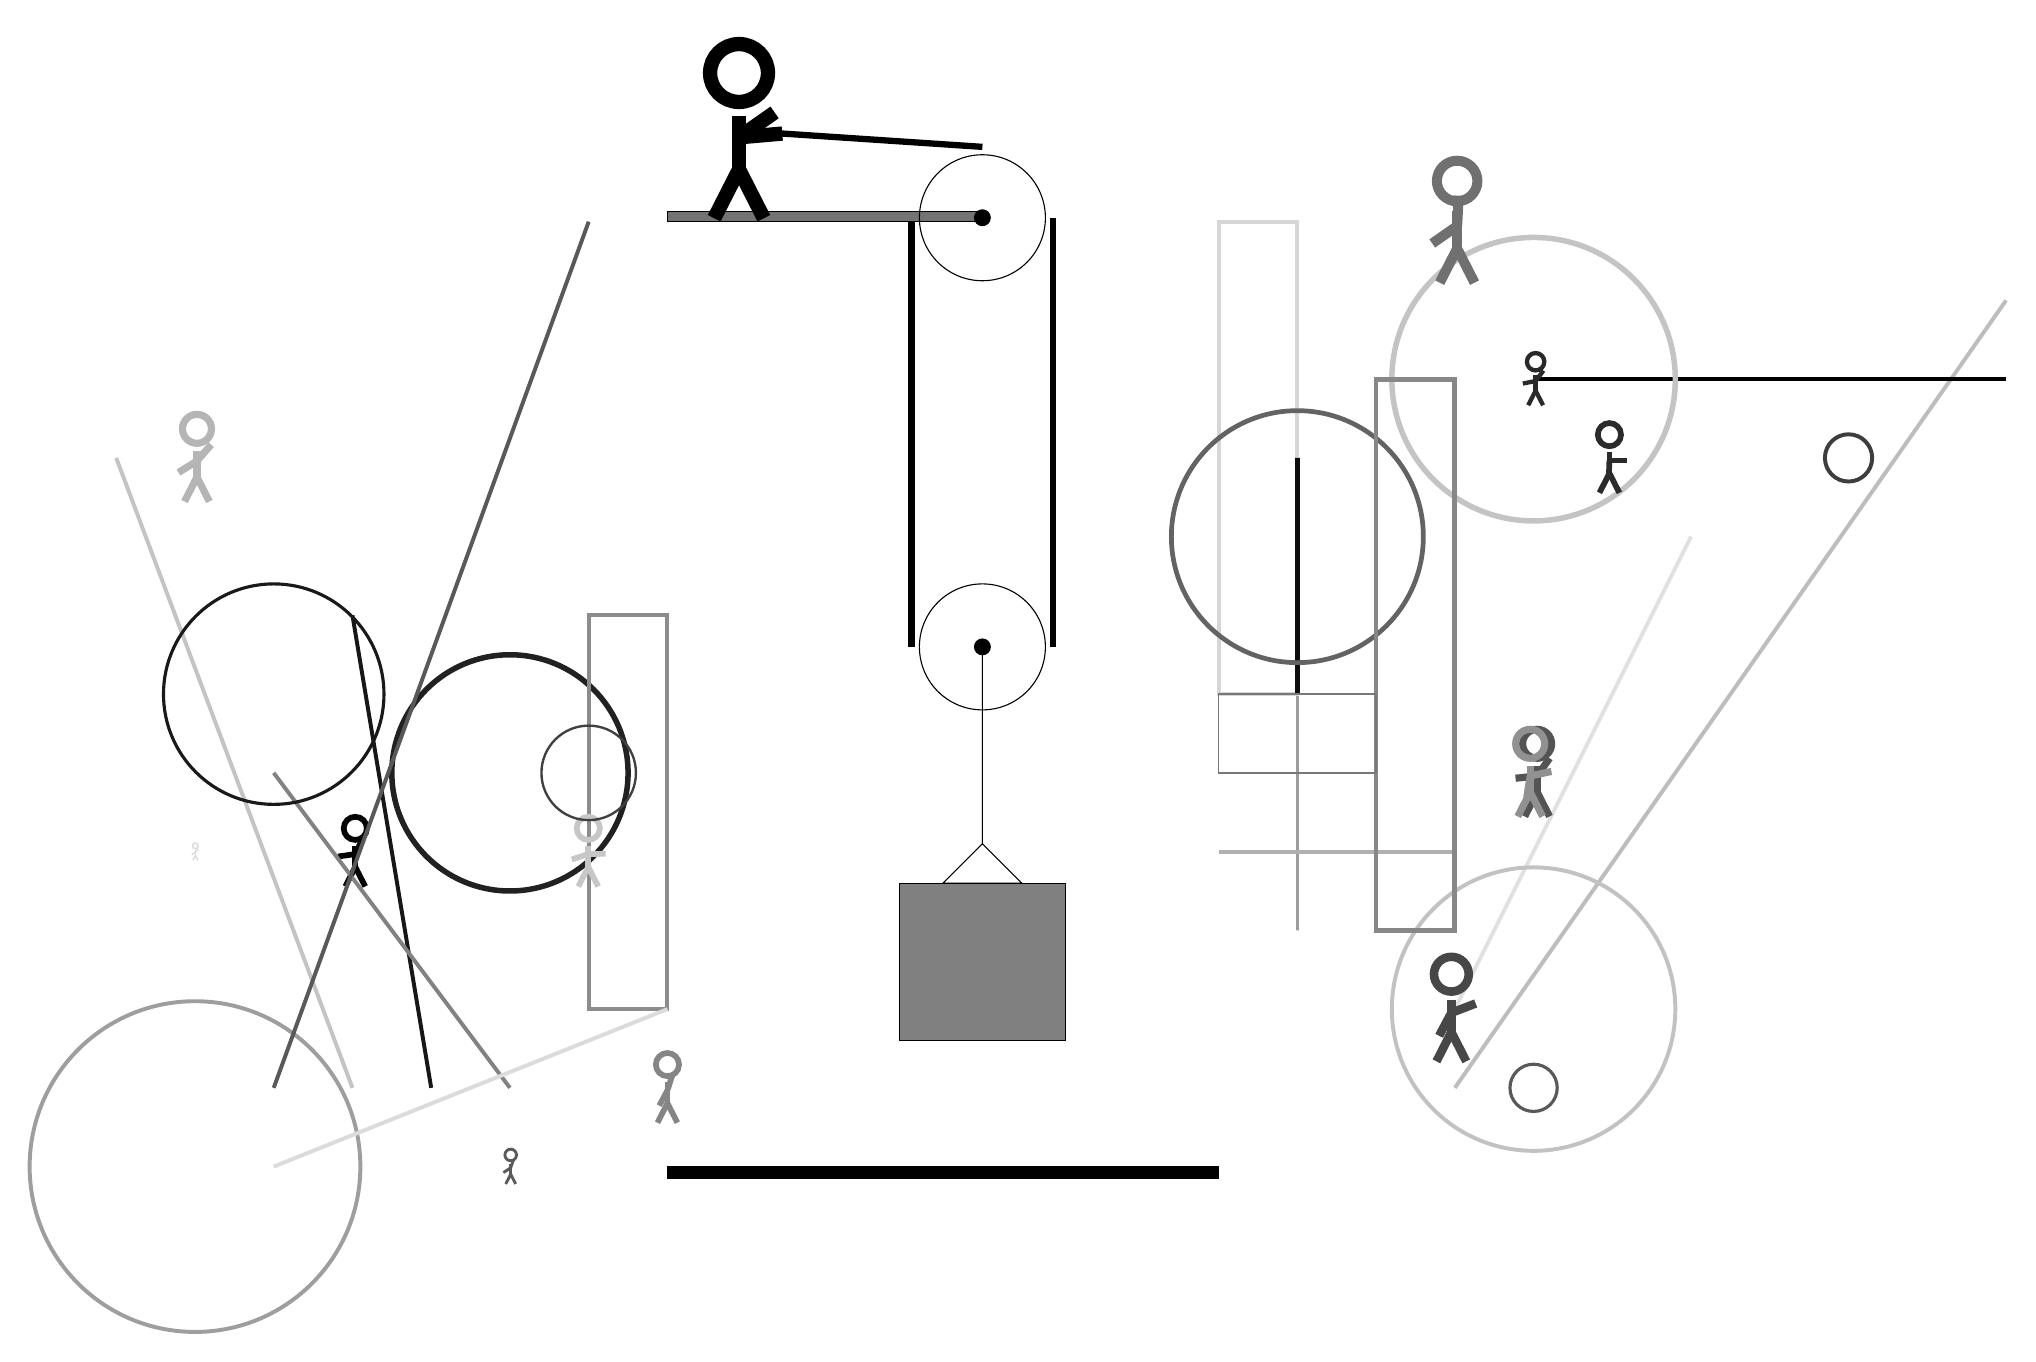
\begin{tikzpicture}
			%%%%% START %%%%%
			
			\draw[fill=black!55] (-2, 9) rectangle (2, 9.125);
			
			\draw (2, 3.6) circle (0.8);
			\draw[fill=black] (2, 3.6) circle (0.1);
			
			\draw (2, 9.05) circle (0.8);
			\draw[fill=black] (2, 9.05) circle (0.1);
			
			\draw (2, 3.6) -- (2, 1.1) -- (1.5, 0.6) -- (2.5, 0.6) -- (2, 1.1);
			\draw[fill=black!50] (0.95, 0.6) rectangle (3.05, -1.4);
			
			\draw[line width=0.4mm, color=black!39] (6, 3) rectangle (6, 0);
			
			\draw[line width=0.5mm, color=black!16] (5, 3) rectangle (6, 9);
			\draw[line width=0.5mm, color=black!91](-6, 4) -- (-5, -2);
			\node[line width=0.6mm, color=black!14] at (-8, 1) {\Strichmaxerl[1][34][52]};
			\node[line width=0.3mm, color=black!98] at (-6, 1) {\Strichmaxerl[4][8][65]};
			\draw[line width=0.5mm, color=black!26](8, -2) -- (15, 8);
			\draw [line width=0.7mm, color=black!87](-4, 2) circle (1.5);
			\draw[line width=0.5mm, color=black!45] (-3, 4) rectangle (-2, -1);
			\draw[line width=0.7mm, color=black!95] (6, 3) rectangle (6, 6);
			\node[line width=0.6mm, color=black!48] at (-2, -2) {\Strichmaxerl[4][62][72]};
			\draw[line width=0.5mm, color=black!100](9, 7) -- (15, 7);
			\draw [line width=0.6mm, color=black!61](6, 5) circle (1.6);
			\node[line width=0.5mm, color=black!22] at (-3, 1) {\Strichmaxerl[4][18][1]};
			
			\draw[line width=0.5mm, color=black!23](-6, -2) -- (-9, 6);
			\node[line width=0.5mm, color=black!29] at (-8, 6) {\Strichmaxerl[5][32][49]};
			\node[line width=0.7mm, color=black!65] at (-4, -3) {\Strichmaxerl[2][33][71]};
			
			\draw [line width=0.7mm, color=black!23](9, 7) circle (1.8);
			\draw[line width=0.5mm, color=black!12](8, -1) -- (11, 5);
			\node[line width=0.7mm, color=black!67] at (9, 2) {\Strichmaxerl[5][6][55]};
			\draw [line width=0.3mm, color=black!75](-3, 2) circle (0.6);
			\draw [line width=0.5mm, color=black!24](9, -1) circle (1.8);
			\draw[line width=0.5mm, color=black!49](-7, 2) -- (-4, -2);
			\draw[line width=0.5mm, color=black!31](5, 1) -- (8, 1);
			\node[line width=0.6mm, color=black!56] at (8, 9) {\Strichmaxerl[7][35][87]};
			\node[line width=0.4mm, color=black!84] at (9, 7) {\Strichmaxerl[3][11][53]};
			
			\draw [line width=0.4mm, color=black!90](-7, 3) circle (1.4);
			\node[line width=0.4mm, color=black!43] at (9, 2) {\Strichmaxerl[5][81][12]};
			\draw [line width=0.5mm, color=black!38](-8, -3) circle (2.1);
			\draw[line width=0.5mm, color=black!14](-7, -3) -- (-2, -1);
			\draw[line width=0.6mm, color=black!47] (7, 0) rectangle (8, 7);
			\node[line width=0.2mm, color=black!83] at (10, 6) {\Strichmaxerl[4][88][0]};
			
			\draw[line width=0.2mm, color=black!53] (5, 3) rectangle (7, 2);
			\draw[line width=0.5mm, color=black!65](-3, 9) -- (-7, -2);
			\node[line width=0.5mm, color=black!72] at (8, -1) {\Strichmaxerl[6][62][21]};
			\draw [line width=0.5mm, color=black!76](13, 6) circle (0.3);
			\draw [line width=0.4mm, color=black!65](9, -2) circle (0.3);
			
			\draw[line width=0.8mm] (1.1, 9) -- (1.1, 3.6);
			\centerarc[line width=0.8mm](2, 3.6)(180:360:0.9);
			\draw[line width=0.8mm](2.9, 3.6) -- (2.9, 9.05);
			\centerarc[line width=0.8mm](2, 9.05)(0:90:0.9);
			\draw[line width=0.8mm](2, 9.95) -- (-1, 10.15);
			
			\node at (-1, 10.15) {\Strichmaxerl[10][-175][35]};
			
			\draw[fill=black] (-2, -3) rectangle (5, -3.15);
			
			%%%%% END %%%%%
		\end{tikzpicture}
	\end{figure}	
\end{document}